\documentclass{ximera}
\input{../preamble.tex}

 \title{Review for Exam 2} \license{CC BY-NC-SA 4.0}

\begin{document}

\begin{abstract}
 \end{abstract}
\maketitle

\begin{onlineOnly}
\section*{Review Problems for Exam 2}
\end{onlineOnly}

\begin{exercise}
Let $V=\text{span}\left(\begin{bmatrix}2\\0\\1\end{bmatrix},\begin{bmatrix}0\\1\\1\end{bmatrix}, \begin{bmatrix}-4\\0\\-2\end{bmatrix}\right)$.
Recall that the span of a set of vectors in $\RR^n$ is a subspace of $\RR^n$.  From the choices below select ALL sets that can serve as bases for $V$.
 
\begin{selectAll}
 \choice{$\left\{ \begin{bmatrix}2\\0\\1\end{bmatrix},\begin{bmatrix}0\\1\\1\end{bmatrix}, \begin{bmatrix}-4\\0\\-2\end{bmatrix}\right\}$}
 \choice[correct]{$\left\{ \begin{bmatrix}2\\0\\1\end{bmatrix},\begin{bmatrix}0\\1\\1\end{bmatrix}\right\}$}
 \choice[correct]{$\left\{ \begin{bmatrix}0\\1\\1\end{bmatrix}, \begin{bmatrix}-4\\0\\-2\end{bmatrix}\right\}$}
 \choice{$\left\{ \begin{bmatrix}2\\0\\1\end{bmatrix}, \begin{bmatrix}-4\\0\\-2\end{bmatrix}\right\}$}
 \choice[correct]{$\left\{ \begin{bmatrix}2\\1\\2\end{bmatrix},\begin{bmatrix}0\\1\\1\end{bmatrix}\right\}$}
  \end{selectAll}
\end{exercise}

\begin{exercise}
Let $\mathcal{B}=\left\{ \begin{bmatrix}1\\1\\0\end{bmatrix}, \begin{bmatrix}1\\2\\0\end{bmatrix}, \begin{bmatrix}0\\1\\2\end{bmatrix}\right\}$ be an ordered basis for $\RR^3$.  (Mentally verify that $\mathcal{B}$ is a basis of $\RR^3$.)
 
Let $\vec{v}=\begin{bmatrix}-1\\-3\\2\end{bmatrix}$ be a vector of $\RR^3$ (written with respect to the standard basis of $\RR^3$).
Find the coordinate vector for $\vec{v}$ with respect to $\mathcal{B}$.
 
$$\begin{bmatrix}\answer{2}\\\answer{-3}\\\answer{1}\end{bmatrix}$$
\end{exercise}

\begin{exercise}
Consider matrix $A$ and $\text{rref}(A)$ shown below.
$$A=\begin{bmatrix}1&2&1&0&-1\\1&2&2&3&0\\0&0&1&3&1\end{bmatrix}\rightsquigarrow\begin{bmatrix}1&2&0&-3&-2\\0&0&1&3&1\\0&0&0&0&0\end{bmatrix}=\mbox{rref}(A)$$
Find each of the following:
$$\text{rank}(A)=\answer{2}$$
$$\text{dim}\left(\text{row}(A)\right)=\answer{2}$$
$$\text{dim}\left(\text{col}(A)\right)=\answer{2}$$
$$\text{dim}\left(\text{null}(A)\right)=\answer{3}$$
 
Select an appropriate basis for $\text{row}(A)$.
\begin{multipleChoice}
 \choice{$\left\{ \begin{bmatrix}1&2&1&0&-1\end{bmatrix}, \begin{bmatrix}1&2&2&3&0\end{bmatrix}, \begin{bmatrix}0&0&1&3&1\end{bmatrix}\right\}$}
 \choice{$\left\{ \begin{bmatrix}1&2&0&-3&-2\end{bmatrix}, \begin{bmatrix}0&0&1&3&1\end{bmatrix}, \begin{bmatrix}0&0&0&0&0\end{bmatrix}\right\}$}
  \choice[correct]{$\left\{ \begin{bmatrix}1&2&0&-3&-2\end{bmatrix}, \begin{bmatrix}0&0&1&3&1\end{bmatrix}\right\}$}
 \end{multipleChoice}
 
 Using the algorithm presented in this text, find a basis for $\text{col}(A)$.
 
 $$\left\{\begin{bmatrix}\answer{1}\\\answer{1}\\\answer{0}\end{bmatrix}, \begin{bmatrix}\answer{1}\\\answer{2}\\\answer{1}\end{bmatrix}\right\}$$
 
\end{exercise}

\begin{exercise}
Let $\mathcal{B}=\left\{\vec{v}_1, \vec{v}_2\right\}$ be a basis for the plane depicted below.  Find the coordinate vector for $\vec{x}$ with respect to $\mathcal{B}$.
\begin{center}
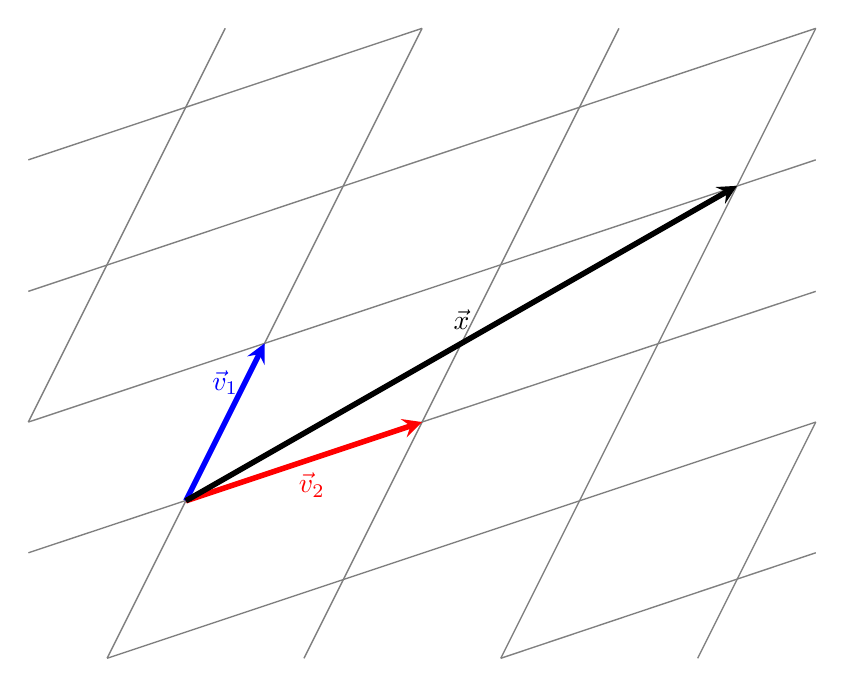
\begin{tikzpicture}[scale=1]
\draw[line width=0.5pt, gray](-2,1)--(0.5,6); 
\draw[line width=0.5pt, gray](-1,-2)--(3,6);
\draw[line width=0.5pt, gray](1.5,-2)--(5.5,6);
\draw[line width=0.5pt, gray](4,-2)--(8,6);
\draw[line width=0.5pt, gray](6.5,-2)--(8,1);
\draw[line width=0.5pt, gray](-2, 4.33)--(3,6);
\draw[line width=0.5pt, gray](-2, 2.66)--(8,6);
\draw[line width=0.5pt, gray](-2, 1)--(8,4.33);
\draw[line width=0.5pt, gray](-2, -0.66)--(8,2.66);
\draw[line width=0.5pt, gray](-1, -2)--(8,1);
\draw[line width=0.5pt, gray](4,-2)--(8,-0.66);
 \draw[line width=2pt,blue,-stealth](0,0)--(1,2);
\draw[line width=2pt,red,-stealth](0,0)--(3,1);
\draw[line width=2pt,-stealth](0,0)--(7,4);
\node[blue] at (0.5, 1.5)  (p2)    {$\vec{v}_1$};
\node[red] at (1.6, 0.2)  (p2)    {$\vec{v}_2$};
\node[] at (3.5, 2.3)  (p2)    {$\vec{x}$};
%\node[] at (-0.2, 0.2)  (p2)    {$\vec{O}$};
 \end{tikzpicture}
 \end{center}
 
 $$\begin{bmatrix}\answer{1}\\\answer{2}\end{bmatrix}$$
 
\end{exercise}

\begin{exercise}
Suppose that $\mathcal{B}_1=\left\{\vec{v}_1, \vec{v}_2\right\}$ is an ordered basis for some subspace $V$ of $\RR^n$.  Let $\mathcal{B}_2=\left\{-\vec{v}_2, -2\vec{v}_1\right\}$.  Verify that $\mathcal{B}_2$ is also an ordered basis for $V$.
 
Let $\vec{w}$ be a vector in $V$.  If the coordinate vector for $\vec{w}$ with respect to $\mathcal{B}_1$ is $\begin{bmatrix}2\\-1\end{bmatrix}$, find the coordinate vector for $\vec{w}$ with respect to $\mathcal{B}_2$.
$$\begin{bmatrix}\answer{1}\\\answer{-1}\end{bmatrix}$$
 
\end{exercise}

\begin{exercise}
 
Determine whether each set, $S$, of vectors is closed under vector addition, and scalar multiplication.
 
Let $S$ be the set of all vectors contained in a sphere of radius 1 centered at the origin.
 
\begin{center}
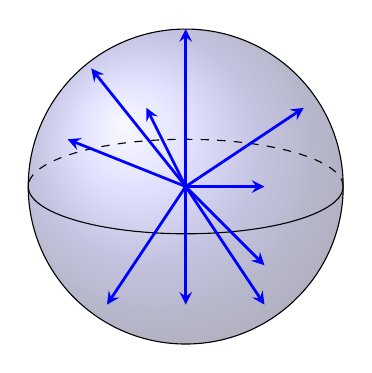
\begin{tikzpicture}
  \shade[ball color = blue!40, opacity = 0.4] (0,0) circle (2cm);
  \draw (0,0) circle (2cm);
  \draw (-2,0) arc (180:360:2 and 0.6);
  \draw[dashed] (2,0) arc (0:180:2 and 0.6);
  \fill[fill=black] (0,0) circle (1pt);
 
  \draw[->,line width=1pt,blue,-stealth](0,0)--(-1.2,1.5);
\draw[->,line width=1pt,blue,-stealth](0,0)--(1,0);
\draw[->,line width=1pt,blue,-stealth](0,0)--(0,-1.5);
\draw[->,line width=1pt,blue,-stealth](0,0)--(1,-1);
\draw[->,line width=1pt,blue,-stealth](0,0)--(-1,-1.5);
\draw[->,line width=1pt,blue,-stealth](0,0)--(1.5,1);
\draw[->,line width=1pt,blue,-stealth](0,0)--(0,2);
\draw[->,line width=1pt,blue,-stealth](0,0)--(-1.5,0.6);
\draw[->,line width=1pt,blue,-stealth](0,0)--(1,-1.5);
\draw[->,line width=1pt,blue,-stealth](0,0)--(-0.5,1);
\end{tikzpicture}
\end{center}
 
\begin{selectAll}
 \choice{$S$ is closed under scalar multiplication.}
 \choice{$S$ is closed under vector addition.}
 \choice[correct]{None of the above.}
 \end{selectAll}
 
Let $S$ be the set of all vectors contained in an infinite double cone.
\begin{center}
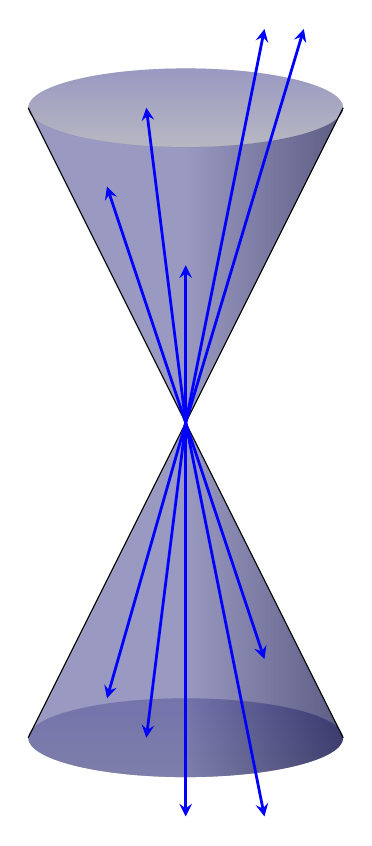
\begin{tikzpicture}
\fill[
  top color=blue!40,
  bottom color=blue!10,
  shading=axis,
  opacity=0.4
  ]
 (0,4) circle (2cm and 0.5cm);
 
 \fill[
  top color=blue!40,
  bottom color=blue!10,
  shading=axis,
  opacity=0.4
  ]
 (0,-4) circle (2cm and 0.5cm);
  
\fill[
  left color=blue!40!white,
  right color=blue!40!black,
  middle color=blue!40,
  shading=axis,
  opacity=0.4
  ]
  (2,-4) -- (0,0) -- (-2,-4) arc (180:360:2cm and 0.5cm);
 
\fill[
  left color=blue!40!white,
  right color=blue!40!black,
  middle color=blue!40,
  shading=axis,
  opacity=0.4
  ]
  (2,4) -- (0,0) -- (-2,4) arc (180:360:2cm and 0.5cm);
   
\draw
  (-2,-4) -- (2,4); 
 
  \draw
  (2,-4) -- (-2,4); 
 
\draw[->,line width=1pt,blue,-stealth](0,0)--(-1,3);
\draw[->,line width=1pt,blue,-stealth](0,0)--(1,5);
\draw[->,line width=1pt,blue,-stealth](0,0)--(0,-5);
\draw[->,line width=1pt,blue,-stealth](0,0)--(1,-3);
\draw[->,line width=1pt,blue,-stealth](0,0)--(-1,-3.5);
\draw[->,line width=1pt,blue,-stealth](0,0)--(1.5,5);
\draw[->,line width=1pt,blue,-stealth](0,0)--(0,2);
\draw[->,line width=1pt,blue,-stealth](0,0)--(-0.5,4);
\draw[->,line width=1pt,blue,-stealth](0,0)--(1,-5);
\draw[->,line width=1pt,blue,-stealth](0,0)--(-0.5,-4);
\end{tikzpicture}
\end{center}
 
\begin{selectAll}
 \choice[correct]{$S$ is closed under scalar multiplication.}
 \choice{$S$ is closed under vector addition.}
 \choice{None of the above.}
 \end{selectAll}
\end{exercise}

\begin{exercise}
Find the dimension of $V$ if $$V=\text{span}\left(\begin{bmatrix}1\\2\\-1\\1\end{bmatrix},\begin{bmatrix}0\\2\\1\\-1\end{bmatrix}, \begin{bmatrix}2\\2\\-3\\3\end{bmatrix}, \begin{bmatrix}-1\\-2\\1\\-1\end{bmatrix}\right) $$
$$\text{dim}(V)=\answer{2}$$
\end{exercise}

\begin{exercise}
 
True or False?  If False, you should come up with a counterexample.  If True, can you give a proof?
 
 \begin{enumerate}
     \item If $V$ is a subspace of $\RR^n$ and $\vec{x}+\vec{y}$ is in $V$, then $\vec{x}$ is in $V$ or $\vec{y}$ is in $V$.
 
 \begin{multipleChoice}
 \choice{True}
 \choice[correct]{False}
 \end{multipleChoice}
 
\item If $V$ is a set in $\RR^n$ such that $c_1{\vec{v}_1}+c_2{\vec{v}_2}$ is in $V$ whenever ${\vec{v}_1}$ and ${\vec{v}_2}$ are in $V$ for any scalars $c_1$, $c_2$, then $V$ is a subspace.
 
 \begin{multipleChoice}
 \choice[correct]{True}
 \choice{False}
 \end{multipleChoice}
 
 \item Every set of four non-zero vectors in $\RR^4$ is a basis.
 
 \begin{multipleChoice}
 \choice{True}
 \choice[correct]{False}
 \end{multipleChoice}
 
 \item $\RR^3$ has a basis of the form $\left\{\vec{x},\vec{x}+\vec{y},\vec{y}\right\}$.
 
 \begin{multipleChoice}
 \choice{True}
 \choice[correct]{False}
 \end{multipleChoice}
 \end{enumerate}
 
  
\end{exercise}

\begin{exercise}
Suppose a linear transformation $T:\RR^2\rightarrow\RR^2$ is such that
$$T\left(\begin{bmatrix}2\\-3\end{bmatrix}\right)=\begin{bmatrix}1\\0\end{bmatrix}$$
$$T\left(\begin{bmatrix}-1\\7\end{bmatrix}\right)=\begin{bmatrix}2\\1\end{bmatrix}$$
Then,
$$T\left(\begin{bmatrix}1\\4\end{bmatrix}\right)=\begin{bmatrix}\answer{3}\\\answer{1}\end{bmatrix}$$
 
 \end{exercise}

 \begin{exercise}
Find the standard matrix $M$ of a linear transformation $T_M:\RR^3\rightarrow \RR^2$ if
$$T\left(\begin{bmatrix}1\\1\\0\end{bmatrix}\right)=\begin{bmatrix}3\\0\end{bmatrix};\quad T\left(\begin{bmatrix}0\\1\\1\end{bmatrix}\right)=\begin{bmatrix}1\\4\end{bmatrix};\quad T\left(\begin{bmatrix}1\\0\\1\end{bmatrix}\right)=\begin{bmatrix}2\\2\end{bmatrix}$$
 
$$M=\begin{bmatrix}\answer{2} & \answer{1} & \answer{0}\\\answer{-1} &\answer{1} & \answer{3}\end{bmatrix}$$
 
 \end{exercise}

 \begin{exercise}
Suppose that an invertible linear transformation $T:\RR^2\rightarrow \RR^2$ is such that
$$T\left(\begin{bmatrix}3\\-1\end{bmatrix}\right)=\begin{bmatrix}4\\-7\end{bmatrix};\quad T\left(\begin{bmatrix}2\\1\end{bmatrix}\right)=\begin{bmatrix}-5\\4\end{bmatrix}$$
 
Find the vector whose image under $T$ is $\begin{bmatrix}3\\-10\end{bmatrix}$
 
$$T\left(\begin{bmatrix}\answer{8}\\\answer{-1}\end{bmatrix}\right)=\begin{bmatrix}3\\-10\end{bmatrix}$$
 
 \end{exercise}

 \begin{exercise}
 
True or False?  If False, you should come up with a counterexample.  If True, can you give a proof?
 
 \begin{enumerate}
 \item $T : \RR^2 \to \RR^2$, given by $T(x, y) = (x, -y)$, is a linear transformation.
 
 \begin{multipleChoice}
 \choice[correct]{True}
 \choice{False}
 \end{multipleChoice}
 
 \item $T : \RR^n \to \RR$, given by $T(\vec{x}) = \vec{x} \cdot \vec{z}$ for some fixed vector $\vec{z} \in \RR^n$, is a linear transformation.
 
 \begin{multipleChoice}
 \choice[correct]{True}
 \choice{False}
 \end{multipleChoice}
 
\item $T : \RR \to \RR$, given by $T(x) = x^2$, is a linear transformation.
 
 \begin{multipleChoice}
 \choice{True}
 \choice[correct]{False}
 \end{multipleChoice}
 
 \item Let $T : \RR^n \to \RR^m$ be a linear transformation and let $\vec{v}_{1}, \dots, \vec{v}_{k}$ denote vectors in $\RR^n$.  If $\{T(\vec{v}_{1}), \dots, T(\vec{v}_{k})\}$ is linearly independent, then $\{\vec{v}_{1}, \dots, \vec{v}_{k}\}$ is also linearly independent.
 
 \begin{multipleChoice}
 \choice[correct]{True}
 \choice{False}
 \end{multipleChoice}
 
 \item Let $T : \RR^2 \to \RR^2$ be a linear transformation and suppose $\vec{v}_{1}, \vec{v}_{2}$ denote vectors in $\RR^2$.  If $\{\vec{v}_{1}, \vec{v}_{2}\}$ is linearly independent, then $\{T(\vec{v}_{1}), T(\vec{v}_{2})\}$ is also linearly independent.
 
 \begin{multipleChoice}
 \choice{True}
 \choice[correct]{False}
 \end{multipleChoice}
 \end{enumerate}
 
  
\end{exercise}

\begin{exercise}
Let $$A=\begin{bmatrix}2 & 1 & -1 & 3\\1 & 0 & 3 & 1\\1 & 1 & -4 & 2\end{bmatrix}$$
 
Use techniques discussed in \href{https://ximera.osu.edu/linearalgebrav3/LinearAlgebraInteractiveIntro/LTR-0050/main}{Image and Kernel of a Linear Transformation} to find the basis for the kernel and the image of the linear transformation, $T_A$, induced by $A$.
 
Basis for $\mbox{im}(T_A)$: $\left\{\begin{bmatrix}\answer{2}\\\answer{1}\\\answer{1}\end{bmatrix}, \begin{bmatrix}\answer{1}\\\answer{0}\\\answer{1}\end{bmatrix}\right\}$
 
Basis for $\mbox{ker}(T_A)$: $\left\{\begin{bmatrix}\answer{-3}\\\answer{7}\\1\\0\end{bmatrix}, \begin{bmatrix}\answer{-1}\\\answer{-1}\\0\\1\end{bmatrix}\right\}$
 
 \end{exercise}
\end{document}